%latexmk -pdf -pvc Notes
\documentclass{article}
\setlength{\oddsidemargin}{6pt}
\setlength{\textwidth}{440pt}
\vspace{-8ex}
\usepackage{listings}
\usepackage{color}
\usepackage{graphicx}
\usepackage[left=0.70in, right=0.70in, top=0.50in, left=0.70in, headsep=0pt]{geometry}
\graphicspath{ {./assets/} }

\definecolor{dkgreen}{rgb}{0,0.6,0}
\definecolor{gray}{rgb}{0.5,0.5,0.5}
\definecolor{mauve}{rgb}{0.58,0,0.82}

\lstset{frame=tb,
  language=Java,
  aboveskip=3mm,
  belowskip=3mm,
  showstringspaces=false,
  columns=flexible,
  basicstyle={\small\ttfamily},
  numbers=none,
  numberstyle=\tiny\color{gray},
  keywordstyle=\color{blue},
  commentstyle=\color{dkgreen},
  stringstyle=\color{mauve},
  breaklines=true,
  breakatwhitespace=true,
  tabsize=3
}

\title{CMSC420 Advanced Data Structures}
\begin{document} 
  \author{Michael Li}
  \title{CMSC420 Advanced Data Structures}
  \maketitle
  \tableofcontents
  \newpage
  \noindent \section{Lists}
  \begin{lstlisting}
    init() => initializes list
    get(i) => returns element at index i
    set(i, x) => sets ith element to x
    length() => returns number of elements in the list
    insert(i, x) => insert x prior to element a_{i} (shifts indices after)
    delete(i) => deletes ith element (shift indices after)
  \end{lstlisting}
  Sequential Allocation (Array): when array is full, increase  its size but a constant factor (e.g. 2). Amortized array operations still O(1) \\ \\
  Linked Allocation (Linked List) \\ \\
  Stack(push, pop): on on end of the list \\
  Queue(enqueue, dequeue): insert at tail (end) and remove from head (start) \\
  Deque(combo stack and queue): can isnert and remove from either ends of list\\
  Multilist: multiple lists combined 1 aggregate structure (e.g. ArrayList)\\
  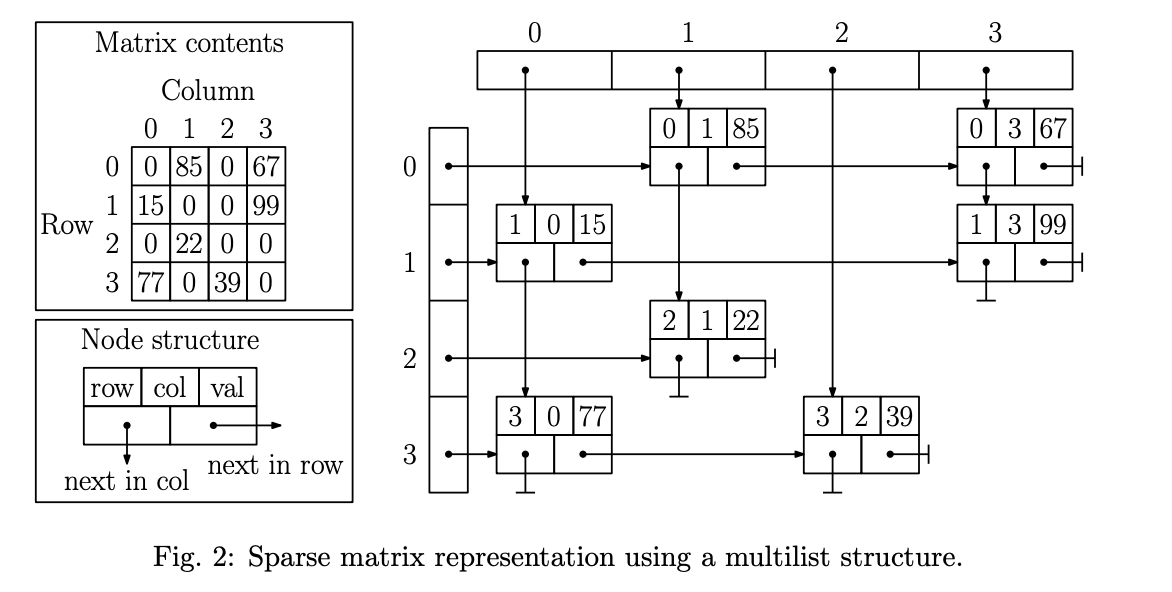
\includegraphics[width=\textwidth]{Fig_2}
  Sparse Matrix: create 2n linked lists for each row and col \\
  \indent Each entry stores a row index, col index, value, next row ptr, and next col ptr
  \newpage
  \noindent\section{Trees}
  Free Tree: connected, undirected graph with no cycles (like MST)\\
  Root Tree: each non-leaf node has $\geq$ 1 children and a single parent (except root)\\
  \indent Aborescence = out-tree \quad Anti-arborescence = in-tree \\
  \indent Depth = max \# of edges of path from root to a node \\ \\
  One way to represent tree is to have a pointer to first child and then a pointer to next sibling \\ \\
  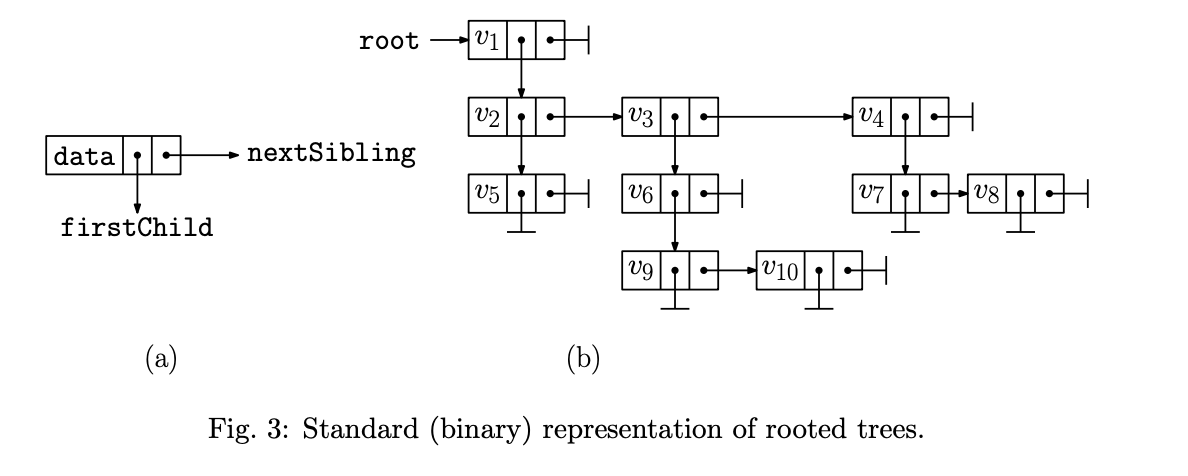
\includegraphics[width=\textwidth]{Fig_3}
  Binary Tree: rooted, ordered tree where each non-leaf node has 2 possible children (left, right) \\ 
  \indent Full Tree: All nodes either have 0 children or 2 children \\
  \indent Can make full binary tree by extending tree by adding external nodes to replace all empty subtrees\\
  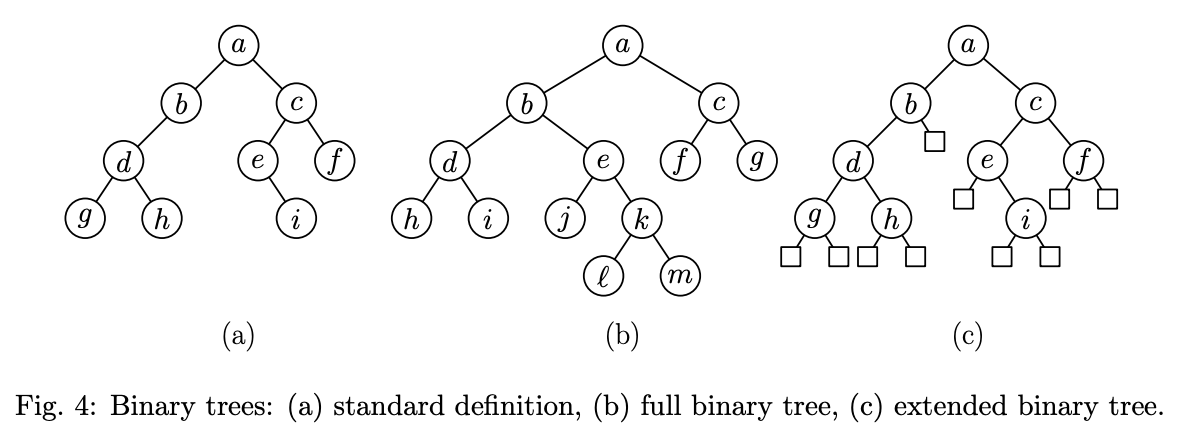
\includegraphics[width=\textwidth]{Fig_4}
  \begin{lstlisting}
    class BinaryTreeNode<E> {
      private E entry;
      private BinaryTreeNode<E> left;
      private BinaryTreeNode<E> right;
      ...
    }
  \end{lstlisting}
 In-order traversal: left, root, right \\
 Pre-order traversal: root, left, right \\ 
 Post-order traversal: left, right, root\\
 If there are n internal nodes in an extended tree, there are n+1 external nodes \\
 \indent Proof by induction: Extended tree binary tree with n internal nodes has n+1 external nodes has 2n+1 total nodes \\
 \indent Let x(n) = number of external nodes given n internal nodes and prove x(n) = n + 1 \\
 \indent Base Case x(0) = 1 a tree with no internal nodes has 1 external node \\
 \indent IH: Assume x(i) = i + 1 for all i $\leq$ n - 1 \\
 \indent IS: let $n_{L}$ and $n_{R}$ be the number of nodes in Left and Right subtrees \\
 \indent x(n) = ($n_{L}$ + 1) + ($n_{R}$ + 1) = (1 + $n_{L}$ + $n_{R}$) + 1 = n + 1 external nodes \\
 \indent so n + 1 (external) + n (internal) = 2n + 1 \\
 \indent Moreover, about 1/2 of nodes of extended Binary Tree are leaf nodes \\
 Threaded Binary Tree: Give null pointers information about where to traverse next \\
 \indent If left-child = null then stores reference to node's inorder predecessor \\
 \indent If right-child = null then stores references to node's inorder successor \\
 \includegraphics[width=\textwidth]{Fig_6}
\end{document}

